% Standalone TikZ figure: Synthetic Data Generation Pipeline
% For Chapter 4: Synthetic Data Generation for Object Detection
\documentclass[tikz,border=10pt]{standalone}
\usepackage{tikz}
\usetikzlibrary{arrows.meta, positioning, shapes.geometric, fit, backgrounds, calc}

\begin{document}
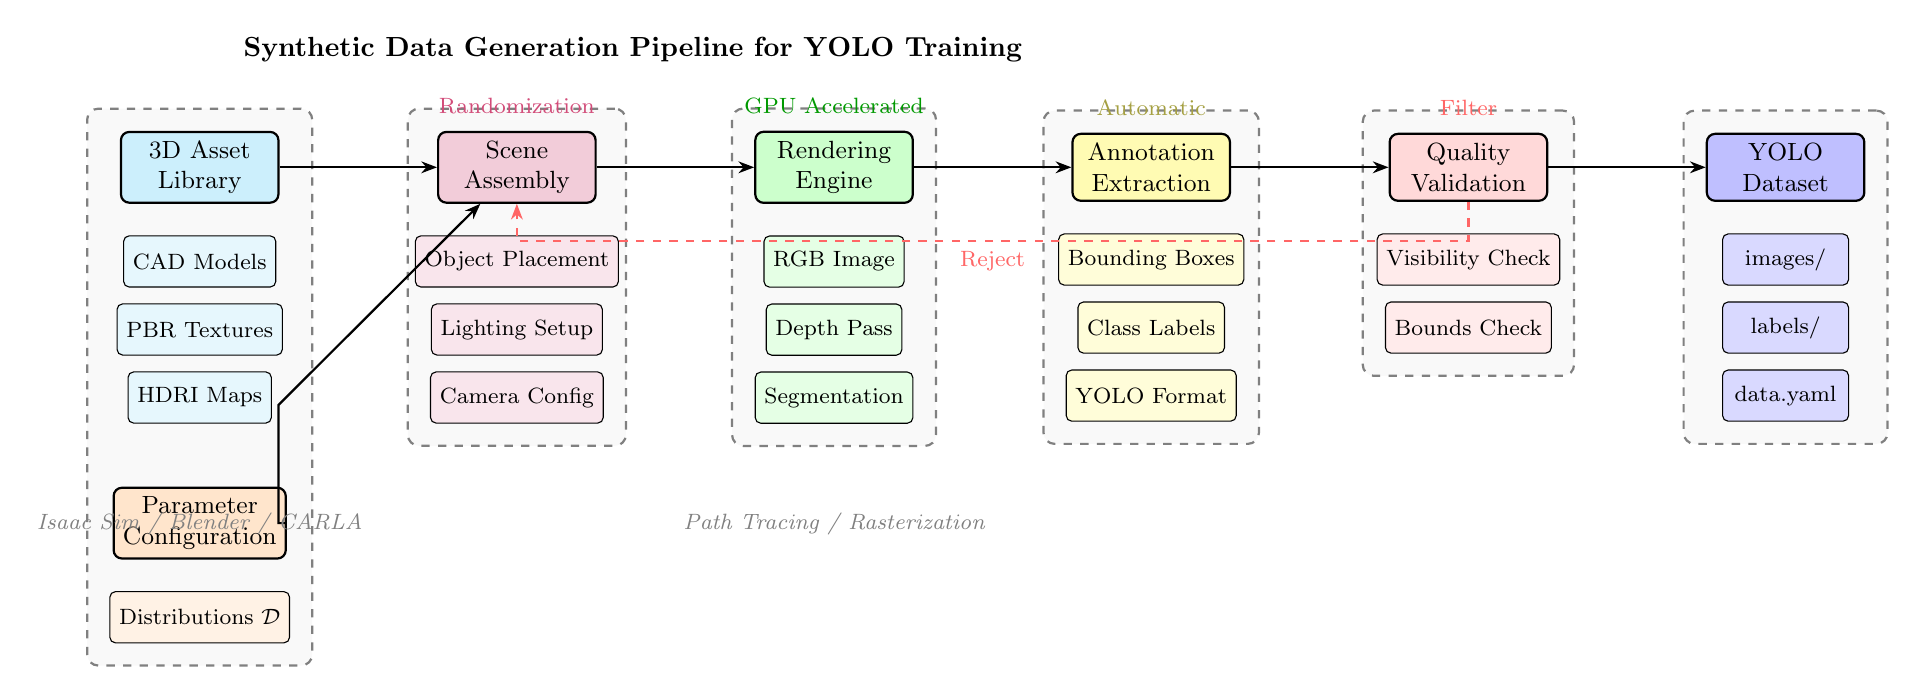
\begin{tikzpicture}[
    node distance=1.0cm and 1.2cm,
    every node/.style={font=\small},
    box/.style={rectangle, draw, thick, minimum width=2.0cm, minimum height=0.85cm, align=center, rounded corners=3pt},
    databox/.style={rectangle, draw, minimum width=1.6cm, minimum height=0.65cm, align=center, rounded corners=2pt, font=\footnotesize},
    arrow/.style={-{Stealth[length=2mm]}, thick},
    label/.style={font=\footnotesize},
    title/.style={font=\bfseries\small}
]

% ============ TITLE ============
\node[title, font=\bfseries] at (5.5, 1.5) {Synthetic Data Generation Pipeline for YOLO Training};

% ============ INPUT STAGE ============
\node[box, fill=cyan!20] (assets) at (0, 0) {3D Asset\\Library};
\node[databox, fill=cyan!10, below=0.4cm of assets] (models) {CAD Models};
\node[databox, fill=cyan!10, below=0.2cm of models] (textures) {PBR Textures};
\node[databox, fill=cyan!10, below=0.2cm of textures] (hdri) {HDRI Maps};

\node[box, fill=orange!20, below=0.8cm of hdri] (config) {Parameter\\Configuration};
\node[databox, fill=orange!10, below=0.4cm of config] (dists) {Distributions $\mathcal{D}$};

% ============ SCENE ASSEMBLY ============
\node[box, fill=purple!20, right=2cm of assets] (scene) {Scene\\Assembly};
\node[databox, fill=purple!10, below=0.4cm of scene] (place) {Object Placement};
\node[databox, fill=purple!10, below=0.2cm of place] (light) {Lighting Setup};
\node[databox, fill=purple!10, below=0.2cm of light] (cam) {Camera Config};

% ============ RENDERING ============
\node[box, fill=green!20, right=2cm of scene] (render) {Rendering\\Engine};
\node[databox, fill=green!10, below=0.4cm of render] (rgb) {RGB Image};
\node[databox, fill=green!10, below=0.2cm of rgb] (depth) {Depth Pass};
\node[databox, fill=green!10, below=0.2cm of depth] (seg) {Segmentation};

% ============ ANNOTATION ============
\node[box, fill=yellow!30, right=2cm of render] (annotate) {Annotation\\Extraction};
\node[databox, fill=yellow!15, below=0.4cm of annotate] (bbox) {Bounding Boxes};
\node[databox, fill=yellow!15, below=0.2cm of bbox] (cls) {Class Labels};
\node[databox, fill=yellow!15, below=0.2cm of cls] (norm) {YOLO Format};

% ============ QUALITY CONTROL ============
\node[box, fill=red!15, right=2cm of annotate] (qc) {Quality\\Validation};
\node[databox, fill=red!8, below=0.4cm of qc] (vis) {Visibility Check};
\node[databox, fill=red!8, below=0.2cm of vis] (bounds) {Bounds Check};

% ============ OUTPUT ============
\node[box, fill=blue!25, right=2cm of qc] (dataset) {YOLO\\Dataset};
\node[databox, fill=blue!15, below=0.4cm of dataset] (imgs) {images/};
\node[databox, fill=blue!15, below=0.2cm of imgs] (labels) {labels/};
\node[databox, fill=blue!15, below=0.2cm of labels] (yaml) {data.yaml};

% ============ ARROWS ============
\draw[arrow] (assets) -- (scene);
\draw[arrow] (config) -| ++(1,1.5) -- (scene);
\draw[arrow] (scene) -- (render);
\draw[arrow] (render) -- (annotate);
\draw[arrow] (annotate) -- (qc);
\draw[arrow] (qc) -- (dataset);

% Rejection loop
\draw[arrow, red!60, dashed] (qc.south) -- ++(0,-0.5) -| node[pos=0.25, below, font=\footnotesize, text=red!60] {Reject} (scene.south);

% ============ FRAMEWORK LABELS ============
\node[font=\footnotesize\itshape, text=gray, below=3.8cm of assets] {Isaac Sim / Blender / CARLA};
\node[font=\footnotesize\itshape, text=gray, below=3.8cm of render] {Path Tracing / Rasterization};

% ============ PROCESS ANNOTATIONS ============
\node[label, above=0.1cm of scene, text=purple!70] {Randomization};
\node[label, above=0.1cm of render, text=green!60!black] {GPU Accelerated};
\node[label, above=0.1cm of annotate, text=yellow!60!black] {Automatic};
\node[label, above=0.1cm of qc, text=red!60] {Filter};

% ============ BACKGROUND GROUPING ============
\begin{scope}[on background layer]
    \node[draw=gray, dashed, thick, rounded corners, fill=gray!5,
          fit=(assets)(textures)(hdri)(config)(dists), inner sep=8pt,
          label={[font=\footnotesize\bfseries, text=gray]above:Inputs}] {};
    \node[draw=gray, dashed, thick, rounded corners, fill=gray!5,
          fit=(scene)(cam), inner sep=8pt,
          label={[font=\footnotesize\bfseries, text=gray]above:Assembly}] {};
    \node[draw=gray, dashed, thick, rounded corners, fill=gray!5,
          fit=(render)(seg), inner sep=8pt,
          label={[font=\footnotesize\bfseries, text=gray]above:Render}] {};
    \node[draw=gray, dashed, thick, rounded corners, fill=gray!5,
          fit=(annotate)(norm), inner sep=8pt,
          label={[font=\footnotesize\bfseries, text=gray]above:Annotate}] {};
    \node[draw=gray, dashed, thick, rounded corners, fill=gray!5,
          fit=(qc)(bounds), inner sep=8pt,
          label={[font=\footnotesize\bfseries, text=gray]above:Validate}] {};
    \node[draw=gray, dashed, thick, rounded corners, fill=gray!5,
          fit=(dataset)(yaml), inner sep=8pt,
          label={[font=\footnotesize\bfseries, text=gray]above:Output}] {};
\end{scope}

\end{tikzpicture}
\end{document}
